\chapter{Obtención de la Vista Minable}\label{chap:2}

Este capítulo se centra en desarrollar las tres primeras fases de la metodología CRISP-DM (comprensión del negocio, comprensión de los datos y preparación de los datos), como parte del proceso KDD, para la obtención de la vista minable que se empleará en la investigación. 


\section{Comprensión del negocio}

El BCC, es la principal entidad financiera de nuestro país. En sus bases de datos se registran todas las operaciones generadas por sus clientes, día tras día. Este aumento de información con el paso del tiempo hace más difícil el análisis de forma manual por parte de los analistas, sobretodo en tareas como la detección de fraude bancario. \\
El objetivo de la institución es determinar qué algoritmo de aprendizaje automático presenta mejor efectividad para la detección de fraude en transacciones bancarias. \\
Como objetivos de la minería, se tienen:
\begin{itemize}
	\item Clasificar las transacciones con respecto a si son fraudulentas o no.
	\item Definir reglas de asociación que determinen los conjuntos de datos más frecuentes cuando se ejecute un fraude. 
	\item Identificar las agrupaciones existentes en las transacciones.
\end{itemize}
Criterios de éxito de la minería:
\begin{itemize}
	\item Obtener un clasificador que acierte como mínimo en un 65\%.
	\item Obtener un modelo de agrupamiento que permita obtener grupos de transacciones de acuerdo a sus características.
	\item Obtener reglas de asociación con un mínimo de confianza de 90\% y un soporte mínimo de 10\%.	
\end{itemize}
En el epígrafe siguiente se procede a la segunda fase de la metodología CRISP-DM: comprensión de los datos.

\section{Comprensión de los datos}

La información necesaria para desarrollar la investigación fue obtenida en el sitio Kaggle, de donde se extrajo una base de datos particionada para su posterior entrenamiento y prueba, en formato Excel (.csv). Esta base de datos es generada por un simulador, siendo un total de 1 852 395 transacciones con 30 atributos. Estas abarcan el periodo del 1 de enero de 2019 al 31 de diciembre de 2020. De estas transacciones, se tiene un total de 9 651 catalogadas como fraudulentas.


\subsection{Descripción de los datos}

A continuación, en la tabla \ref{tabla:descrip-atributos-bd} se describe cada una de las variables de la base de datos utilizada para obtener la vista minable.

	\begin{longtable} {p{3.5cm} p{2cm} c p{2cm} p{6cm}}
		\toprule
		\textbf{Nombre} & \textbf{Tipo} & \textbf{Nulos} & \textbf{Valores distintos} & \textbf{Descripción} \\
		\midrule
		\endfirsthead
		
		\toprule
		\textbf{Nombre} & \textbf{Tipo} & \textbf{Nulos} & \textbf{Valores distintos} & \textbf{Descripción} \\
		\midrule
		\endhead
		
		% aquí añadimos el fondo de todas las hojas, excepto de la última.
		\hline
		\endfoot
		
		% aquí añadimos el fondo de la última hoja.
		\endlastfoot
	
		transdatetrans\_time & Nominal & 0 & 1 819 551 & Fecha y hora de la transacción\\
		\addlinespace
		cc\_num & Numérico & 0 & 999 & Número de tarjeta de crédito del cliente\\
		\addlinespace
		merchant & Nominal & 0 & 693 & Nombre del comerciante \\
		\addlinespace
		category & Nominal & 0 & 14 & Categoría del comerciante \\
		\addlinespace
		amt & Numérico & 0 & 60 616 & Monto de la transacción \\
		\addlinespace
		first & Nominal & 0 & 355 & Nombre del titular de la tarjeta de crédito \\
		\addlinespace
		last & Nominal & 0 & 486 & Apellido del titular de la tarjeta de crédito \\
		\addlinespace
		gender & Nominal & 0 & 2 & Género del titular de la tarjeta de crédito \\
		\addlinespace
		street &  Nominal & 0 & 999 & Calle del titular de la tarjeta de crédito \\
		\addlinespace
		city &  Nominal & 0 & 906 & Ciudad del titular de la tarjeta de crédito \\
		\addlinespace
		state &  Nominal & 0 & 51 & Estado del país del titular de la tarjeta de crédito\\
		\addlinespace
		zip & Numérico & 0 & 985 & Código postal del titular de la tarjeta de crédito \\
		\addlinespace
		lat & Numérico & 0 & 983 & Latitud del titular de la tarjeta de crédito al realizar la transacción\\
		\addlinespace
		long & Numérico & 0 & 983 & Longitud del titular de la tarjeta de crédito al realizar la transacción \\
		\addlinespace
		city\_pop & Numérico & 0 & 891 & Población de la ciudad del titular de la tarjeta de crédito \\
		\addlinespace
		job & Nominal & 0 & 497 & Empleo del titular de la tarjeta de crédito \\
		\addlinespace
		dob & Nominal & 0 & 984 & Fecha de nacimiento del titular de la tarjeta de crédito \\
		\addlinespace
		trans\_num & Nominal & 0 & 1 852 394 & Número de transacción \\
		\addlinespace
		unix\_time & Numérico & 0 & 1 819 583 & Hora de la transacción en formato UNIX \\
		\addlinespace
		merch\_lat & Numérico & 0 & 1 754 157 & Latitud del comerciante \\
		\addlinespace
		merch\_long & Numérico & 0 & 1 809 753& Longitud del comerciante \\
		\addlinespace
		is\_fraud & Numérico & 0 & 2 & Indicador de fraude (Clase objetivo)\\	
		\bottomrule 
		\\
		\caption{Descripción de los atributos de la base de datos}
		\label{tabla:descrip-atributos-bd}
	\end{longtable}


\section{Preparación de los datos}

El objetivo principal de esta fase es la construcción, a partir de los datos originales del dataset, de la vista minable a emplear. En este apartado se realizan las tareas de  limpieza, transformación y selección de datos.

\subsection{Selección, limpieza y transformación de los datos}
Se presentan a continuación los mecanismos utilizados para transformar y limpiar los datos presentes en la base de datos.

\subsubsection{Manipulación de Fecha y hora}
En la base de datos se tiene el atributo \textsf{transdatetrans\_time} que contiene unidas la fecha y la hora. Este atributo se separa en dos nuevos atributos: \textsf{trans\_date} (Fecha) y \textsf{trans\_time} (Hora). Para ello se emplea el nodo \textit{Extract Date\&Time Fields}. Se elimina el atributo \textsf{transdatetrans\_time}. \\
Tras obtener la fecha y hora de las transacciones por separado, se crean los atributos nominales \textsf{Month(name)} y \textsf{Day\_of\_week(name)}, empleando el nodo \textit{Extract Date\&Time Fields}, que contienen el nombre del mes y del día de la semana en que se efectuaron las transacciones, respectivamente.
 Además, se obtienen el atributo nominal \textsf{Time}, cuyos valores están presentes en la tabla \ref{tabla:atributo-time}, a partir del conocimiento de la hora de la transacción. Para esta transformación se emplea el nodo \textit{Rule Engine}.

\begin{table} [H]
	\centering
	\begin{tabular}{p{5cm} p{7cm}}
		\toprule
		\textbf{Valor generado} & \textbf{Significado} \\
		\midrule
		Between 0 and 7 & Transacciones efectuadas entre las 12:00:00 a.m. y las 6:59:59 a.m. \\
		\addlinespace
		Between 7 and 13 & Transacciones efectuadas entre las 7:00:00 a.m. y las 12:59:59 p.m. \\
		\addlinespace
		Between 13 and 21 & Transacciones efectuadas entre la 1:00:00 p.m. y las 20:59:59 p.m. \\
		Between 21 and 0 & Transacciones efectuadas entre las 9:00:00 p.m. y las 11:59:59 p.m. \\
		\bottomrule
	\end{tabular}
	\caption{Descripción de valores generados para el atributo \textsf{Time}}
	\label{tabla:atributo-time}
\end{table}

\subsubsection{Manipulación de Fecha de nacimiento}
El atributo \textsf{dob} presenta la fecha de nacimiento de cada titular. Este atributo se empleó para la creación de los atributos \textsf{age} y \textsf{Age}. El primero, de tipo Integer, contiene la edad del titular, mientras el segundo, un rango de edad, de tipo String. Para esta transformación se emplea el nodo \textit{Rule Engine}. Los valores se encuentran en la tabla \ref{tabla:atributo-age}.

\begin{table} [H]
	\centering
	\begin{tabular}{l l}
		\toprule
		\textbf{Valor generado} & \textbf{Significado} \\
		\midrule
		Teen & Titulares con menos de 18 años de edad \\
		\addlinespace
		Young Adult & Titulares con edad comprendida entre 19 y 25 años \\
		\addlinespace
		Middle-Age & Titulares con edad comprendida entre 26 y 55 años \\ 
		\addlinespace
		Old & Titulares con más de 56 años de edad \\ 
		\bottomrule
	\end{tabular}
	\caption{Descripción de valores generados para el atributo \textsf{Age}}
	\label{tabla:atributo-age}
\end{table}

Tras esta transformación, se eliminan los atributos \textsf{dob} y \textsf{trans\_date}. Este último se elimina puesto a que el atributo \textsf{unix\_time} contiene la misma información.


\subsubsection{Manipulación de Es Fraude:}
Entre los campos numéricos se encuentra el atributo \textsf{is\_fraud} (Es Fraude). Este atributo se convierte a String pues se utiliza como valor nominal. Se emplea el nodo \textit{String Replacer}.
Las transformaciones realizadas fueron:
\begin{itemize}
	\item Transformar el atributo \textsf{is\_fraud} a tipo String.
	\item Sustituir el valor 0 por NO.
	\item Sustituir el valor 1 por SI.
\end{itemize}

\subsubsection{Manipulación de Longitud y Latitud:}
En esta base de datos no se tiene información de los cajeros desde donde se realizaron las transacciones. Sin embargo, entre los campos numéricos se encuentran las variables \textsf{lat} (Latitud) y \textsf{long} (Longitud). Ambas son sometidas a un clustering para determinar los cajeros más cercanos equivalentes al número de clústeres. Se emplea el algoritmo K-Means con K = 890 para semejar a la cantidad de cajeros existentes en Cuba \citep{Hernandez2021}. De este número de cajeros, se asocian 665 como los utilizados. Se le denomina \textsf{atm\_id} a la identificación de los cajeros. En la figura  se presenta el flujo empleado para esta transformación.

\begin{figure}[H]
	\centering
	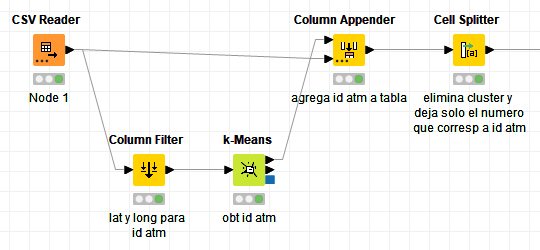
\includegraphics[width=0.8\linewidth]{figuras/tranf-atm}
	\caption{Flujo empleado en la creación del atributo \textsf{atm\_id}}
	\label{fig:tranf-atm}
\end{figure}

\subsubsection{Manipulación de Monto}
La variable numérica \textsf{amt}, correspondiente al monto de transacción, es transformada a tipo nominal para poder ser empleada en algoritmos que solo admiten este tipo de variables. El nuevo atributo es nombrado \textsf{Amount}. En la tabla se muestran los resultados tras emplear el nodo \textit{Rule Engine}.

\begin{table} [H]
	\centering
	\begin{tabular}{l l}
		\toprule
		\textbf{Valor generado} & \textbf{Significado} \\
		\midrule
		Low Amount & Transacciones mayores a \$0 y menores a \$64.99 \\
		\addlinespace
		Average & Transacciones mayores a \$65 y menores a \$89.99 \tablefootnote{El monto promedio, tras ejecutar el nodo \textsf{Statistics}, es cerca de los \$75. Por dicho motivo se establece una variación del monto promedio entre los \$65 y \$90.} \\
		\addlinespace
		High Amount & Transacciones mayores a \$90 y menores a \$9 999.99 \\ 
		\addlinespace
		Very high amount & Transacciones mayores a \$10 000 \\ 
		\bottomrule
	\end{tabular}
	\caption{Descripción de valores generados para el atributo \textsf{Amount}}
	\label{tabla:atributo-amount}
\end{table}

\section{Selección de los datos}

Tras la ejecución de las transformaciones, se eliminaron algunas de las variables redundantes en la base de datos. No obstante, existen variables que contienen un gran conjunto de valores únicos y que no son útiles para la aplicación de los algoritmos. Por tal motivo se decidió eliminar, en total, las variables: \textsf{cc\_num, merchant, first, last, street, city, zip, city, zip, city\_pop, dob, trans\_num, trans\_date} y \textsf{trans\_time}. La vista minable resultante se muestra en la figura \ref{fig:vista-minable}.
\begin{figure}[H]
	\centering
	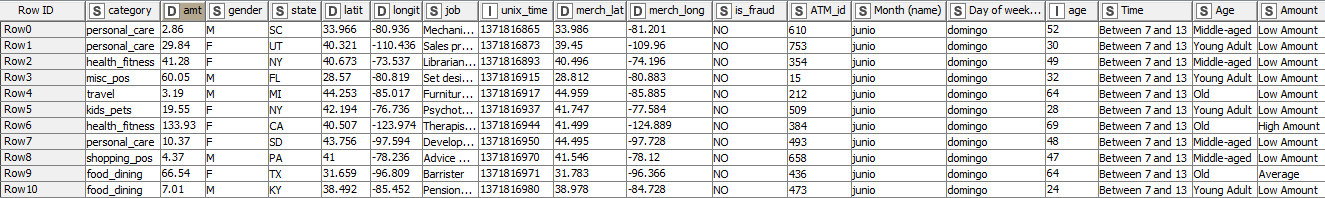
\includegraphics[width=1\linewidth]{figuras/vista-minable}
	\caption{Resultado de la Vista Minable}
	\label{fig:vista-minable}
\end{figure}

\section{Conclusiones parciales}

% Cada conclusión tiene que estar sustentada en el cuerpo del capítulo.

Una vez terminado el capítulo se arriban a las siguientes conclusiones:

\begin{enumerate}
	\setlength\itemsep{0em}
	\item No se encontraron valores nulos o perdidos en la base de datos.
	\item Existían numerosas variables poco relevantes para el análisis de los datos, tales como el nombre y apellidos del titular de la tarjeta de crédito, las cuales fueron eliminadas.
	\item Hubo varias transformaciones de atributos que conllevaron a la creación de otros más importantes, como es el caso del identificador del cajero automático.
	\item Se obtuvo una vista minable en función de las características de cada transacción.
\end{enumerate}
\pagebreak

